
%(BEGIN_QUESTION)
% Copyright 2012, Tony R. Kuphaldt, released under the Creative Commons Attribution License (v 1.0)
% This means you may do almost anything with this work of mine, so long as you give me proper credit

Two instrument technicians are arguing over how to build a current transformer (CT) circuit to facilitate convenient measurement of CT secondary current without having to break the circuit open, because they both recognize the danger of an open-circuited CT.

$$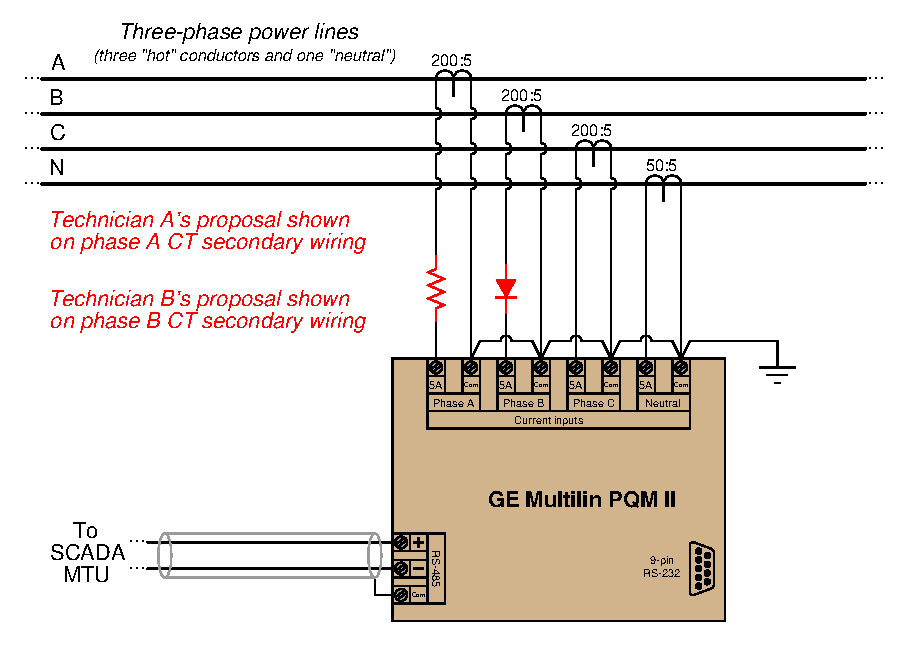
\includegraphics[width=15.5cm]{i02131x01.eps}$$

Technician ``A'' proposes installing a {\it shunt resistor} (on the order of 1 milliohm resistance) in series with the CT secondary wiring, so that a technician may connect an AC millivoltmeter across the shunt and use the measured voltage to calculate current.  Technician ``B'' proposes installing a {\it diode} in series with the CT secondary wiring, so that a technician may connect an AC ammeter across the diode and measure current (just like in a 4-20 mA loop circuit).  

Do you think either of these proposals are valid?  Is one better than the other?  Explain your answer in detail.

\underbar{file i02131}
%(END_QUESTION)





%(BEGIN_ANSWER)

Half-credit for identifying the better proposal, and half-credit for explaining why the other proposal would not work.

\vskip 10pt

Technician ``A'' has the best proposal.  A shunt resistor of low value would permit indirect measurement of current (by measuring AC millivoltage and calculating current using Ohm's Law).  

Technician ``B's'' idea will not work, and in fact is dangerous.  Since the current in question is AC and not DC, the diode will cause the CT to be open-circuited every half-cycle, which of course will cause high voltages to develop across the CT secondary winding every half-cycle with much damage and hazard to nearby personnel!

%(END_ANSWER)





%(BEGIN_NOTES)

{\bf This question is intended for exams only and not worksheets!}

%(END_NOTES)


